\section{Bootstrap e CSS Personalizado}
%---------------------------------------------------------------------[ Início ]
\begin{frame}[allowframebreaks, fragile,t]{Bootstrap e CSS Personalizado}
    \begin{itemize}
      \item  Bootstrap (\verb!http://getbootstrap.com/!) é framework CSS desenvolvido
        pelo Twitter e disponibilizado na forma de código de aberto. Para incluí-lo
        em uma aplicação Rails é necessário utilizar a gem \alert{bootstrap-sass}.
      \begin{exampleblock}{\tiny\textbf{caminho: }\url{Gemfile}}
        \lstinputlisting[style=RubyInputStyle, basicstyle=\tiny\ttfamily, firstline=14, lastline=14]{rails/codigos/microblog_4/Gemfile}
      \end{exampleblock}
      
      \item É necessário executar o \verb!bundle install! para que a nova gem seja corretament
        instalada.
      \begin{exampleblock}{Exemplo:}
          \begin{lstlisting}[style=BashInputStyle]
$ cd ~/workspace/blog
$ bundle install
          \end{lstlisting}
      \end{exampleblock}
      
      \item O CSS personalizado da aplicação pode ser colocado em um arquivo que 
        deverá ser armazenado na pasta \verb!app/assets/stylesheets/!. 
      \begin{exampleblock}{Exemplo:}
          \begin{lstlisting}[style=BashInputStyle]
$ cd ~/workspace/blog
$ touch app/assets/stylesheets/custom.css.scss
          \end{lstlisting}
      \end{exampleblock}
      
      \item O framework \verb!bootstrap! deverá ser incluído no arquivo \verb!custom.css.scss!
      utilizando o comando \alert{@import}. Para que o servidor reconheça o bootstrap, é necessário
      reinicializá-lo teclando \verb!CTRL+C! e digitando \verb!rails s! na pasta raiz da aplicação.
      \begin{exampleblock}{\tiny\textbf{caminho: }\url{app/assets/stylesheets/custom.css.scss}}
        \lstinputlisting[style=RubyInputStyle, basicstyle=\tiny\ttfamily, firstline=1, lastline=2]{rails/codigos/microblog_4/app/assets/stylesheets/custom.css.scss}
      \end{exampleblock}
      
      \item O primeiro conjunto de propriedades CSS, que será incluído no arquivo, formatará
        alguns elementos gerais da página, como, por exemplo, a tag \verb!<body>!.
      \begin{exampleblock}{\tiny\textbf{caminho: }\url{app/assets/stylesheets/custom.css.scss}}
        \lstinputlisting[style=RubyInputStyle, basicstyle=\tiny\ttfamily, firstline=4, lastline=21]{rails/codigos/microblog_4/app/assets/stylesheets/custom.css.scss}
      \end{exampleblock}
      
      \item O segundo conjunto de propriedades CSS, que será incluído no arquivo, formatará
        alguns elementos relacionados à tipografia da página, como, por exemplo, o tag \verb!<h1>!
      \begin{exampleblock}{\tiny\textbf{caminho: }\url{app/assets/stylesheets/custom.css.scss}}
        \lstinputlisting[style=RubyInputStyle, basicstyle=\tiny\ttfamily, firstline=23, lastline=41]{rails/codigos/microblog_4/app/assets/stylesheets/custom.css.scss}
      \end{exampleblock}
      
      \item O último conjunto de propriedades CSS, que será incluído no arquivo, formatará
        o logo da página que neste caso é a palavra "Microblog". 
      \begin{exampleblock}{\tiny\textbf{caminho: }\url{app/assets/stylesheets/custom.css.scss}}
        \lstinputlisting[style=RubyInputStyle, basicstyle=\tiny\ttfamily, firstline=42, lastline=55]{rails/codigos/microblog_4/app/assets/stylesheets/custom.css.scss}
      \end{exampleblock}
      
    \end{itemize}
\end{frame} 
%---------------------------------------------------------------------[ Início ]
\begin{frame}[allowframebreaks, fragile,t]{Página Principal}
       \begin{figure}[h!]
        \centering
        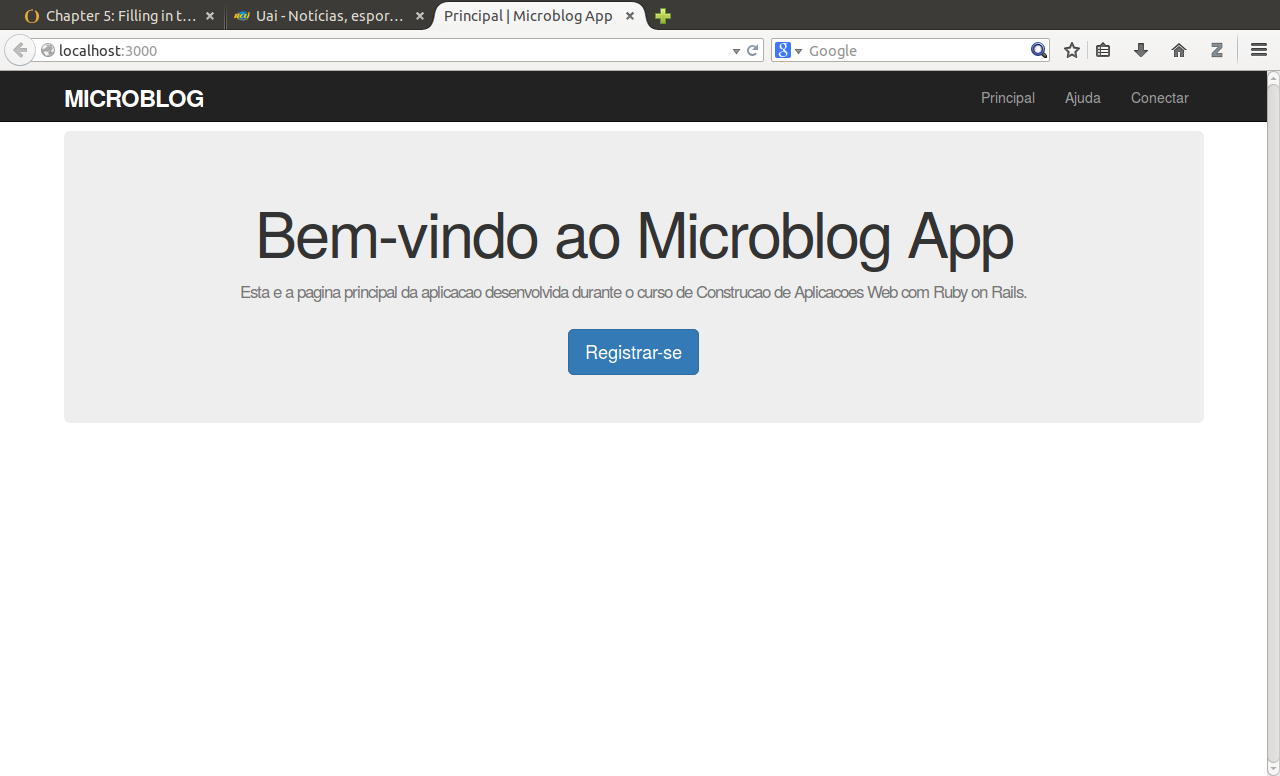
\includegraphics[width=0.90\textwidth]{rails/imagens/tela-principal.png}
      \end{figure}
\end{frame}